\chapter[Rubidium Production in Massive AGB Stars]{\textbf{Rubidium Production in \\ Massive AGB Stars}}
\label{ch:Rb}

% \cite{Iliadis2020} for mutual information (and the original 1950's paper)

% In some cases, the MACS of radioactive nuclei can be measured by the activation technique (Ref. Kappeler 2011), because of the ability to use extremely small sample masses. Howerver, measurements of the MACS for the branch point at $^{85}$Kr is hampered by the high specific activity. (The data obtained via activation usually represent the respective MACS values at kT = 25 keV and have to be extrapolated to higher and lower temperatures by means of theoretical data)

\section{Introduction}

\section{Rubidium Overabundance} \label{sec:Rb_Overabundance}

% Show the Kr - Rb s-process path

% Significant overabundance (predicted vs. observed solar system abundance) of Rb, even accounting for r-process contribution(?).

% 22Ne(a,n)25Mg reaction rate should be sensitive to the Sr/Rb abundance ratio

% Theoretical motivation for 86Rb(n,g)87Rb measurement... (but the real motivation is the RESULT of my sensitivity study of the predicted Rb/Sr abundance ratio with respect to the 22Ne(a,n)25Mg neutron source)

\section{s-Process Reaction Network Methodology}

%

\subsection{The Reaction Network}

% Description of the nuclei / reactions in the network (rates from Starlib) and their initial abundances.
% Start off with the simple 47.5% 22Ne, 47.5% 4He, and 5% 85Rb case.
% Then then solar system abundances case, where 1H --> 4He and 12C+13C --> 14N

\subsection{Reaction Rate Sensitivities}

\subsubsection{Method 1: Manually Varying the 22Ne(a,n) Rate}

\subsubsection{Method 2: Monte Carlo}

% Explanation of the Monte Carlo reaction network calculations

% Explanation of the Spearman, Pearson, and mutual information statistics

    \begin{figure}[t]
        \centering
        \begin{subfigure}[b]{0.495\textwidth}
            \centering
            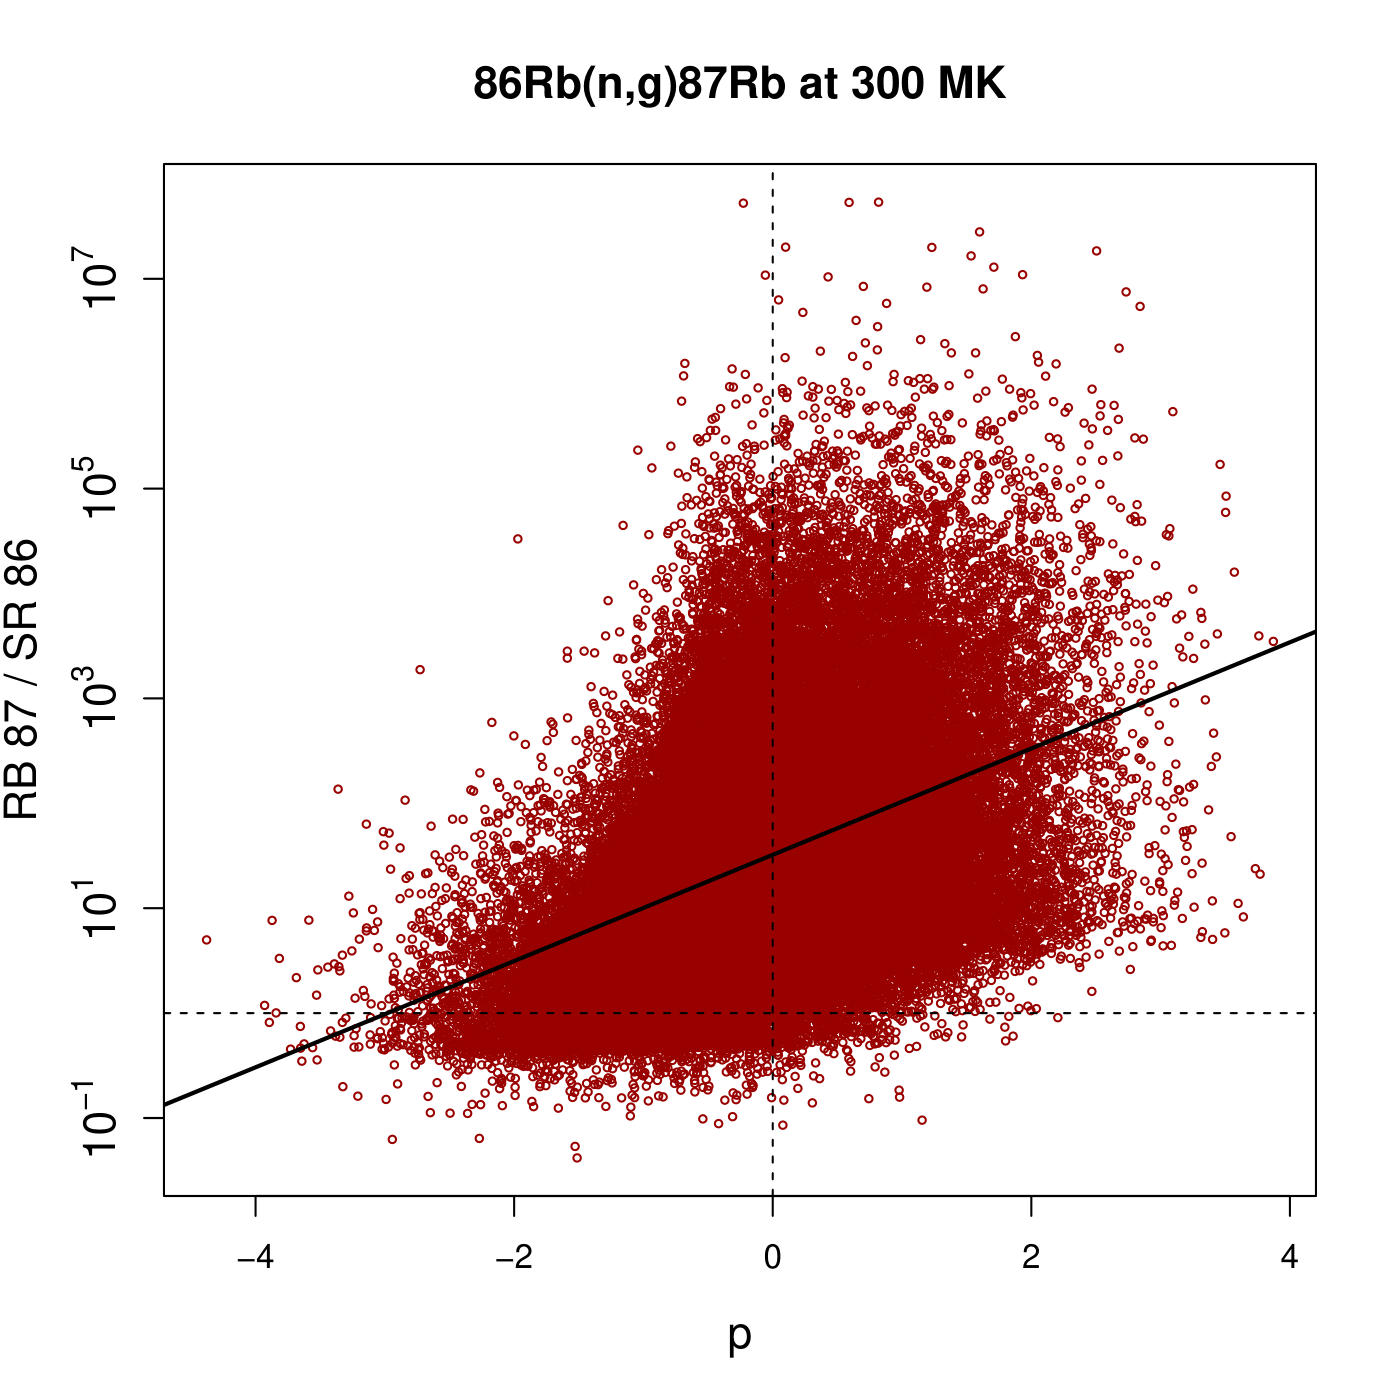
\includegraphics[width=\textwidth]{Chapter-3/figs/CorrRB87SR86_86Rb_n_g_87Rb_300MK.png}  
        \end{subfigure}
        \hfill
        \begin{subfigure}[b]{0.495\textwidth}  
            \centering 
            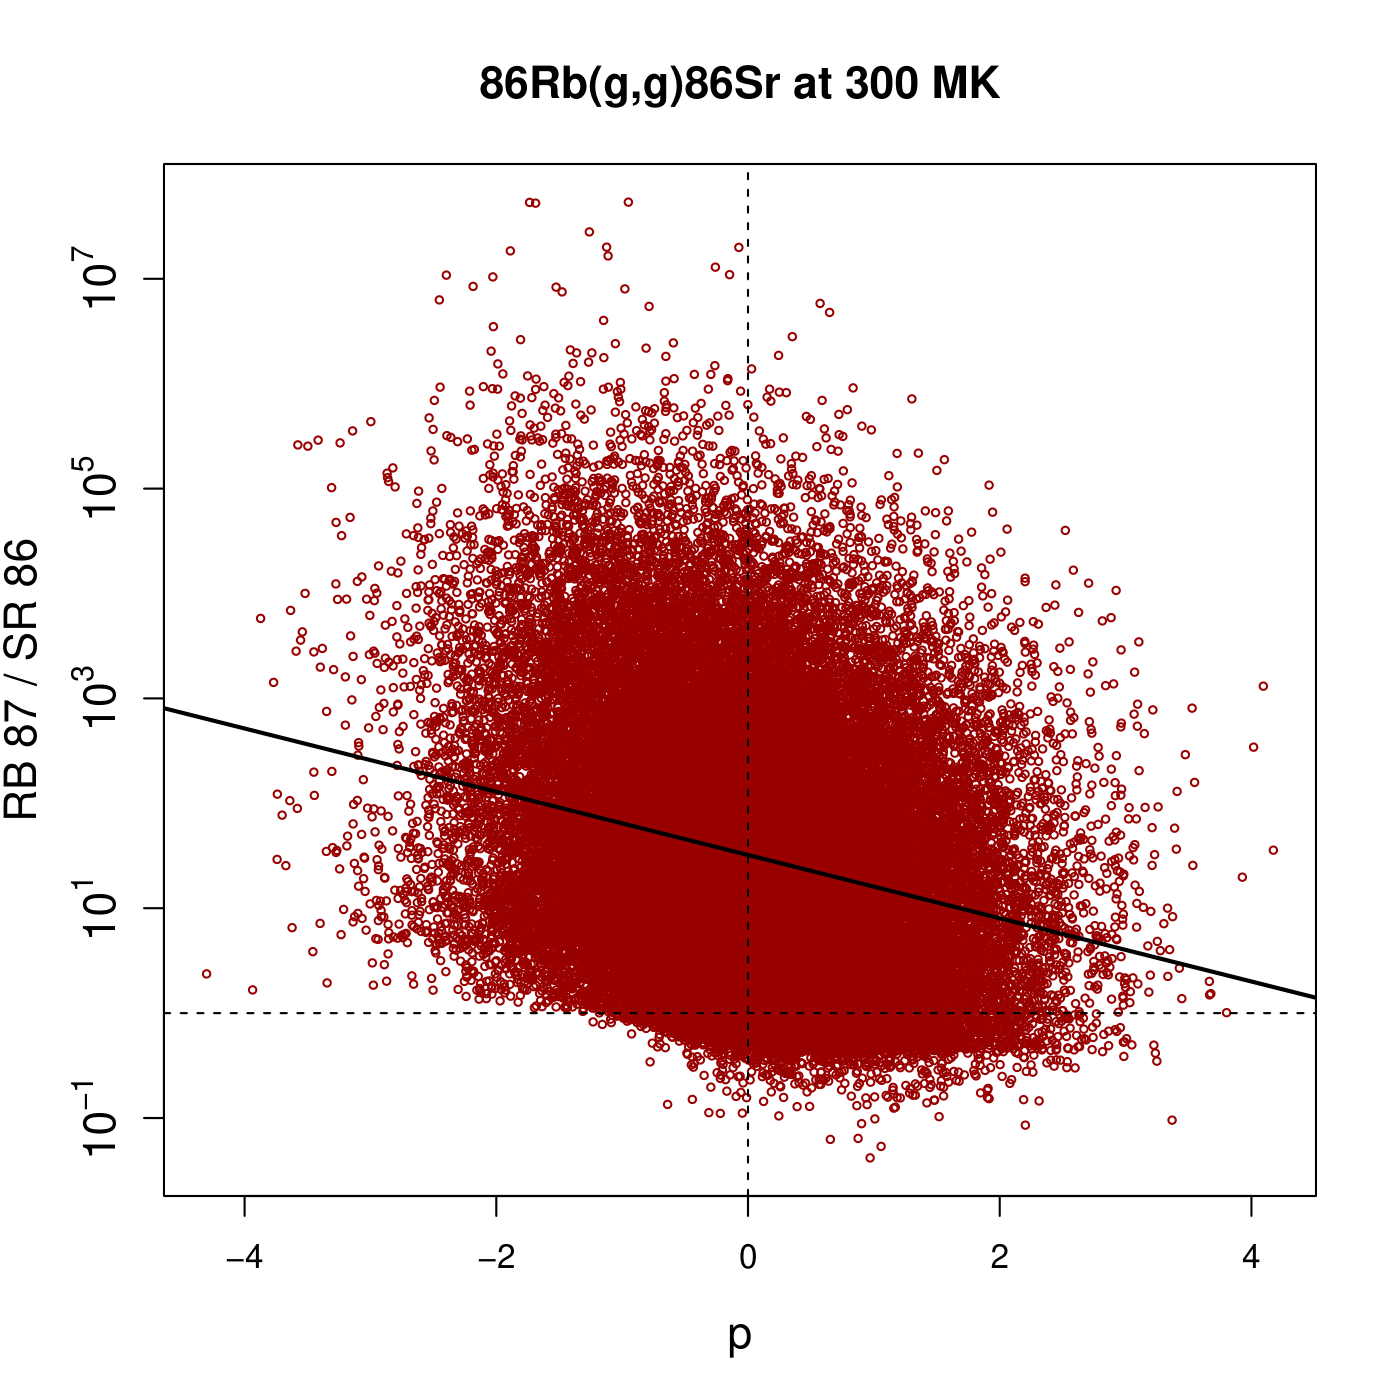
\includegraphics[width=\textwidth]{Chapter-3/figs/CorrRB87SR86_86Rb_g_g_86Sr_300MK.png}
        \end{subfigure}
        %\vskip\baselineskip
        \begin{subfigure}[b]{0.495\textwidth}   
            \centering 
            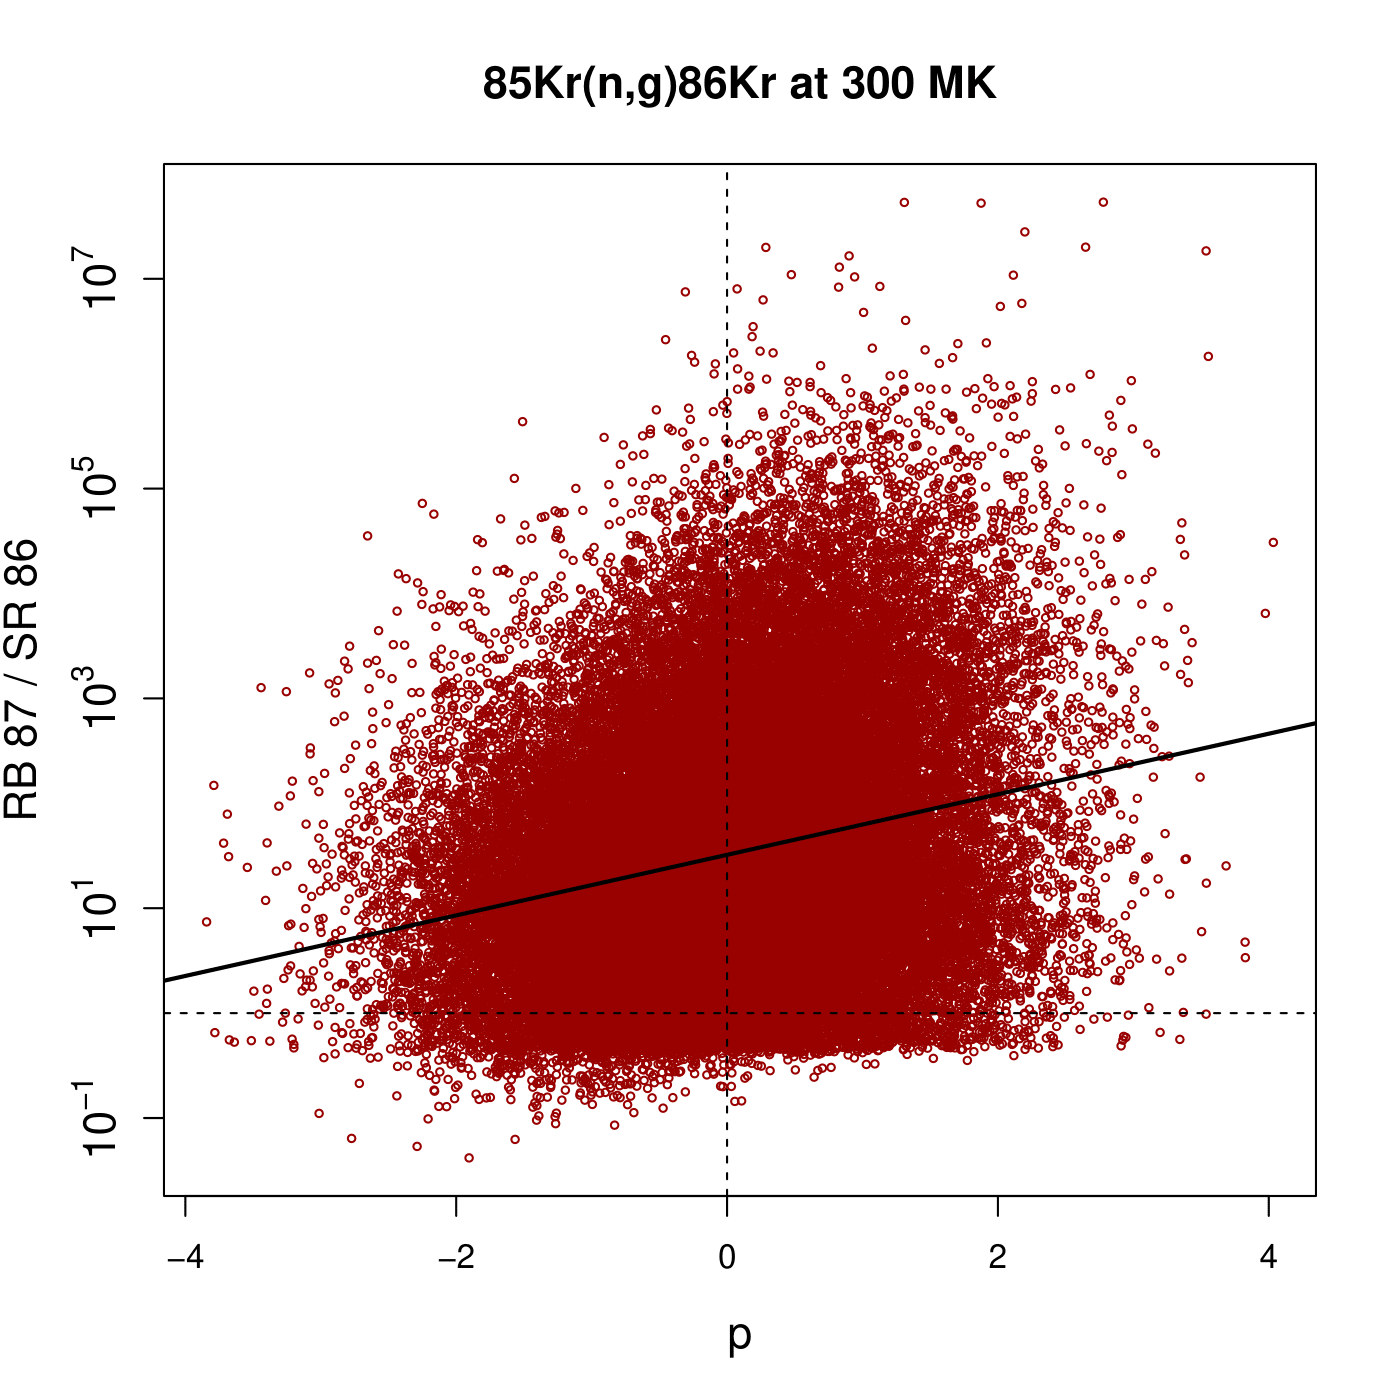
\includegraphics[width=\textwidth]{Chapter-3/figs/CorrRB87SR86_85Kr_n_g_86Kr_300MK.png}
        \end{subfigure}
        \hfill
        \begin{subfigure}[b]{0.495\textwidth}   
            \centering 
            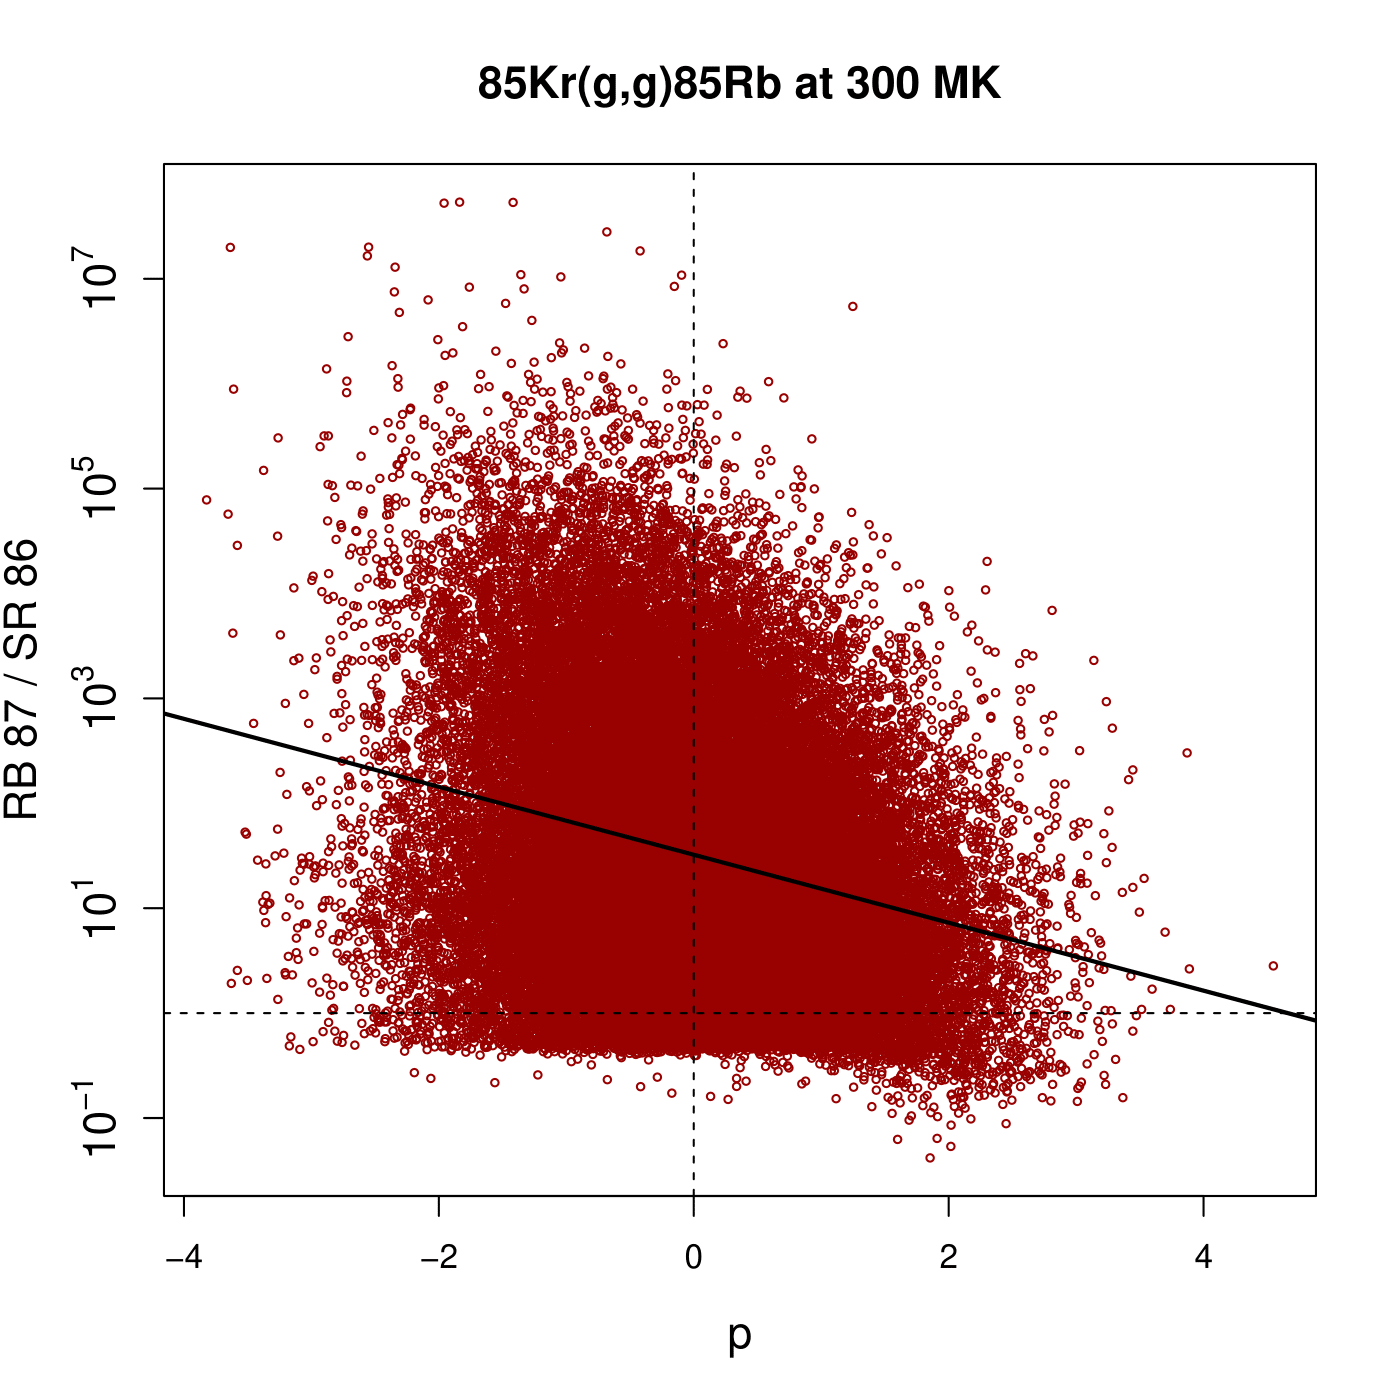
\includegraphics[width=\textwidth]{Chapter-3/figs/CorrRB87SR86_85Kr_g_g_85Rb_300MK.png}
        \end{subfigure}
        \caption{\label{}Here's my caption!} 
    \end{figure}

\section{Re}

\subsection{Abundance Evolution}

% Abundance evolution plots of 87Rb, 88Sr, Kr isotopes, 4He, 14N, 13C, etc.

\begin{figure}[t]
\begin{tikzpicture}[scale=1.0, every node/.style={transform shape}]
\node at (0,0) {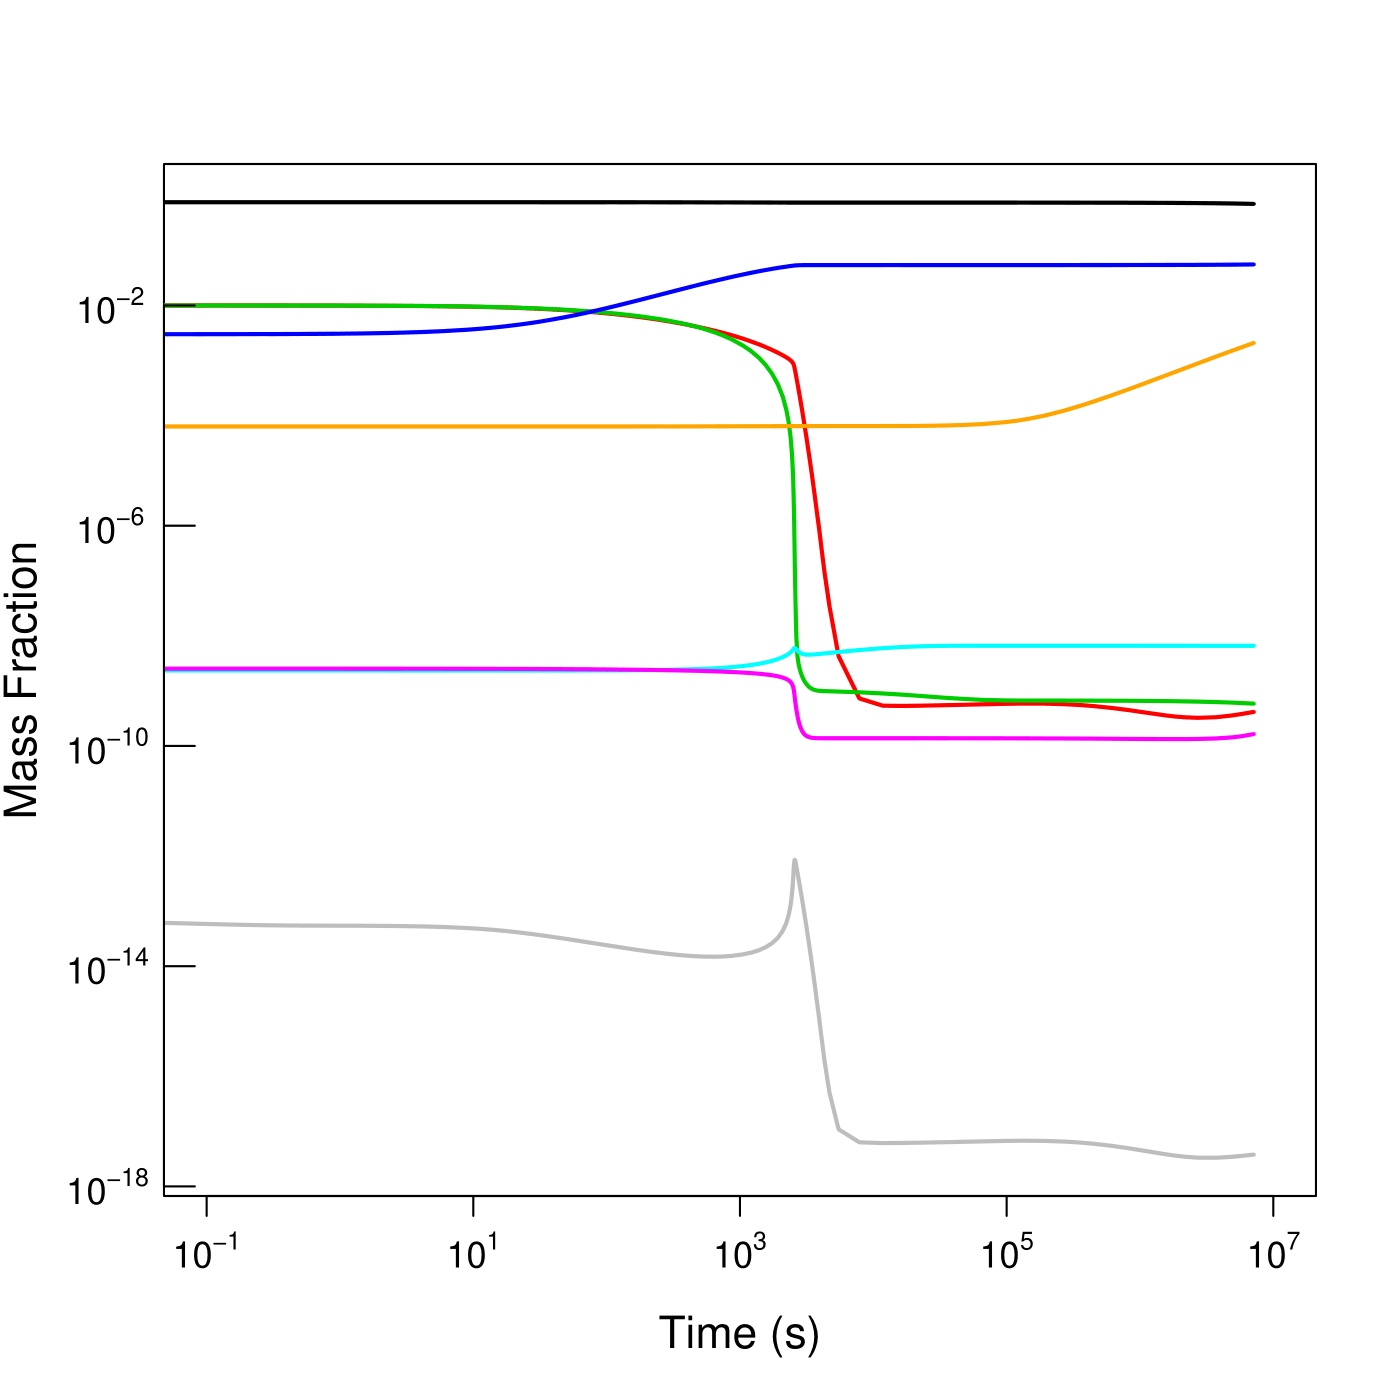
\includegraphics[width=6.5in]{Chapter-3/figs/abund_300MK.png}};
\node at (-1.5,5.6) {$^{4}$He};
\node at (1.8,2) {$^{13}$C};
\node at (0.7,2) {$^{14}$N};
\node at (3,4.75) {$^{16}$O};
\node at (5,3.2) {$^{22}$Ne};
\node at (4,1.0) {$^{87}$Rb};
\node at (4,-0.8) {$^{86}$Sr};
\node at (1.75,-3.5) {$n$};
\node[draw] at (-3,-5) {$T = 300$ MK, $\rho = 10^{3}$ $\mathrm{g}/\mathrm{cm}^{3}$};
\end{tikzpicture}
\caption{\label{fig:abund_evol}The abundance evolution of key nuclei related to the s-process branching at $^{86}$Rb for a single network calculation simulating the conditions during a single AGB thermal pulse. The $T$, $\rho$, and $X_{\mathrm{last}}(^{4}\mathrm{He})$ parameters are 300 MK, $10^{3}$ $\mathrm{g}/\mathrm{cm}^{3}$, and 0.7, respectively, where the initial mass fraction of $^{4}$He was 0.75.}
\end{figure}